% Paper for CS 472/572 (Unsupervised Learning), Fall 2026.
% Build: `make paper` from the repository root, or `latexmk -pdf main.tex` here.
% Figures are read from ../reports/figures/ so the paper always shows the committed results.

\documentclass[10pt,twocolumn]{article}

\usepackage[letterpaper,margin=0.75in,columnsep=0.25in]{geometry}
\usepackage[T1]{fontenc}
\usepackage{mathptmx}
\usepackage{microtype}
\usepackage{amsmath}
\usepackage{graphicx}
\usepackage{booktabs}
\usepackage{xcolor}
\usepackage[font=small,labelfont=bf]{caption}
\usepackage[numbers,sort&compress]{natbib}
\usepackage[hidelinks]{hyperref}

\graphicspath{{../reports/figures/results/}{../reports/figures/}}

% Sections still to be written. Each stub lists what the section must say,
% the numbers it needs and the files they come from. Delete the stub once
% the section is drafted; `make paper` prints how many are left.
\definecolor{stubcolor}{HTML}{8A3B12}
\newenvironment{stub}[1]
  {\par\smallskip\noindent\color{stubcolor}\small\textbf{To write (#1).}\ }
  {\par\smallskip}

\newcommand{\K}{\ensuremath{K}}

\title{Co-occurring conditions in a national sample of autistic children vary along two continuous axes}
\author{Chris Reger \and Haley Berger\\[2pt]
  \small School of Informatics, Computing, and Cyber Systems, Northern Arizona University\\
  \small \texttt{github.com/Naalu/nsch-autism-subtypes}}
\date{}

\begin{document}
\maketitle

\begin{abstract}
\begin{stub}{both, about 150 words, last}
Problem: autism covers very different children, and subtype studies from clinics report three or four groups, rarely checked in new children or against a continuous alternative. Data: 8,891 autistic children aged 6 to 17 in the National Survey of Children's Health 2016 to 2024, 18 parent-reported conditions, 2025 held out. Method: latent class model fit by EM in our own code, checks fixed in advance, latent trait models on the same likelihood scale, every check rerun on simulated data. Findings: (1) four profiles, the combinations of high and low on a developmental-language axis and a psychiatric axis, reproduce across years (ARI 0.71), in 2025 (0.79) and under resampling (Jaccard 0.91); (2) a smooth two-dimensional continuum with no classes reproduces about as well, while four real classes reproduce far better, and two dimensions fit better and predict new years as well as eight classes; (3) severity tracks position on the developmental axis, not class. Caveat: parent report, one time point.
\end{stub}
\end{abstract}

\section{Introduction}
\label{sec:intro}

Autism is one diagnosis for children whose lives look very different. One child has no speech and an intellectual disability; another is in honors classes and is being treated for anxiety and depression. Much of that difference lies in the conditions that come with autism, and co-occurring conditions are a natural place to look for subtypes: groups of children who share a pattern and might share a cause, a course or a treatment.

Studies that have looked report three or four groups, usually a developmental or language group, a psychiatric or behavioral group, a small group with high rates of everything, and a large group with few conditions \citep{doshivelez2014,vargason2019,montgomery2023,litman2025}. Two problems make these findings hard to read. The first is that they are rarely checked. Of 156 autism subtyping studies reviewed by \citet{agelink2021}, 9\% repeated the analysis in an independent sample and 13\% with a second method. The second is that a clustering method finds groups whether or not groups exist. \citet{bauer2003,bauer2004} showed that mixture models recover several classes from data generated by a single continuous population, so ``the model chose $K$ classes'' is not evidence that there are $K$ kinds of children. The usual checks do not settle this either: we show below that a partition of a smooth continuum also reproduces in new samples.

This paper asks both questions of a national survey. We fit a latent class model to 18 parent-reported conditions in 8,891 autistic children aged 6 to 17 from the National Survey of Children's Health (NSCH), 2016 to 2024, and hold out the 2025 survey. The checks and their pass lines were fixed before the first model was fit. We then fit continuous latent trait models to the same data on the same likelihood scale, and we run every replication check on data simulated from each alternative, so that a passing score can be read against what a continuum with no classes would score.

Three findings follow. First, the four profiles that clinic studies report are present, as the four combinations of high and low on a developmental-language axis and a psychiatric axis, and the partition reproduces across survey years, in 2025, within age bands and under resampling. Second, a four-way cut of a smooth two-dimensional continuum reproduces about as well, while data with four real classes reproduce much better; the two-dimensional model also fits better than any class model and predicts new years as well as eight classes. Third, parent-rated severity rises along the developmental axis and does not jump at the class borders. The four profiles are reproducible regions of a map and a useful summary of it. They are not four kinds of children.

The contributions are a from-scratch implementation of the latent class model and its checks; a subtype analysis of co-occurring conditions in a nationally representative sample, with a held-out year; and a calibration of the standard replication checks against simulated data with and without classes, which applies to any subtype study that relies on them.

\section{Related work}
\label{sec:related}

\paragraph{Subtypes from co-occurring conditions.}
\citet{doshivelez2014} clustered diagnosis-code histories of about 4,900 patients at one hospital and found three small distinct groups (seizure, multisystem, psychiatric) and one large unresolved group, with a replication sample from a second region. \citet{lingren2016} reported psychiatric, developmental and seizure groupings in 20,658 hospital records. \citet{vargason2019} applied $k$-means to insurance claims for 3,278 young children and found high rates of everything (24\%), developmental delay (27\%) and low rates (50\%). \citet{montgomery2023} found four groups ordered by support need in 1,151 children from the Australian Autism Biobank, and \citet{litman2025} fit a generative mixture model to more than 5,000 SPARK participants and reported four classes (social and behavioral challenges 37\%, mixed with developmental delay 19\%, moderate challenges 34\%, broadly affected 10\%) that replicated in a second cohort and differed in genetic signal. Across these studies the recurring contrasts are a developmental or language group, a psychiatric or behavioral group and a small high-burden group; the number of groups varies with the inputs and the method.

\paragraph{Validation.}
\citet{agelink2021} distilled the ways a subtype can be validated into a seven-item checklist. External validation on variables not used for clustering was common (88\% of studies); independent replication (9\%), a second method (13\%) and parallel measures (6\%) were rare, and no study used all seven. Our checks follow the checklist (Section~\ref{sec:checks}). Stability under resampling is a separate tradition: \citet{benhur2002} and \citet{lange2004} choose the number of clusters by how well clusterings agree across subsamples, and \citet{hennig2007} gives thresholds for when a single cluster is stable. Current guidance on latent class analysis treats the number of classes as a judgment made from several indices together \citep{masyn2013,nylundgibson2018}.

\paragraph{Types or dimensions.}
\citet{bauer2003,bauer2004} showed that classes can stand in for continuous variation and that fit indices alone cannot tell the two apart. \citet{lubke2006} and \citet{markon2006} showed that fitting class and factor models to the same data on the same likelihood scale can, and \citet{lubke2005} proposed factor mixture models that allow both. Meta-analyses of taxometric studies in personality and psychopathology find dimensional structure about five times as often as categorical \citep{haslam2012,haslam2020}. For core autism traits, \citet{kim2019} found correlated dimensions fit caregiver ratings best in 3,825 clinic-referred youth, and \citet{wittkopf2023} found that BIC preferred dimensions for observation data but that factor scores were multimodal, and argued for a hybrid. We found no study that makes the comparison for co-occurring conditions. On the genetic side, \citet{zhang2025} found that common-variant autism genetics splits into two modestly correlated factors, one tied to earlier diagnosis and early communication difficulty and the other to later diagnosis, adolescent behavioral and emotional difficulty, ADHD and mental health. \citet{lombardo2019} argue that categorical and dimensional descriptions of autism heterogeneity need not exclude each other.

\paragraph{This study.}
The NSCH is a nationally representative survey with state-level samples \citep{ghandour2018}, used before to estimate the prevalence of parent-reported autism \citep{kogan2018} but not, as far as we found, to look for subtypes. Its class shares are population estimates rather than descriptions of a clinic sample. Its inputs are weaker than a clinic's: parent report of a provider's diagnosis, 18 yes/no items and one time point, which limits what it can say about any one child and rules out temporal and predictive validation.

\section{Data}
\label{sec:data}

\paragraph{Survey.}
The NSCH is a yearly household survey run by the Census Bureau for the Maternal and Child Health Bureau. A household is sampled by address, one child is selected, and a parent or caregiver answers a questionnaire about that child online or on paper \citep{ghandour2018}. Each child carries a survey weight, the number of US children that child stands for. We use the ten public topical files from 2016 to 2025, 431,222 children in all.

\paragraph{Selection.}
We keep children aged 6 to 17 whose parent reports that a doctor or other health care provider has told them the child has autism and that the child currently has it. ``Currently'' leaves out children whose diagnosis was later ruled out, and children aged 6 to 17 answer the same questionnaire items on conditions and are old enough for most to have been diagnosed. This gives 9,710 children for 2016 to 2024 and 1,660 for 2025 (Table~\ref{tab:sample}). The 2025 file was released on October 5, 2026; it was processed with the other years, but no model was fit to it and no modeling choice used it until the forward test in Section~\ref{sec:checks}.

\begin{table}[t]
\centering
\caption{Children per survey year. Selected: aged 6 to 17 with current autism. Complete: no missing condition flag, the sample the models are fit to. 2025 is held out.}
\label{tab:sample}
\small
\begin{tabular}{lrrrr}
\toprule
Year & All children & Aged 6--17 & Selected & Complete \\
\midrule
2016 & 50,212 & 35,718 & 1,008 & 922 \\
2017 & 21,599 & 15,438 & 494 & 456 \\
2018 & 30,530 & 21,954 & 687 & 619 \\
2019 & 29,433 & 21,259 & 693 & 643 \\
2020 & 42,777 & 30,636 & 1,030 & 953 \\
2021 & 50,892 & 30,173 & 1,085 & 982 \\
2022 & 54,103 & 34,362 & 1,355 & 1,248 \\
2023 & 55,162 & 33,638 & 1,464 & 1,333 \\
2024 & 51,375 & 37,534 & 1,894 & 1,735 \\
\midrule
2016--2024 & 386,083 & 260,712 & 9,710 & 8,891 \\
2025 & 45,139 & 33,039 & 1,660 & 1,505 \\
\bottomrule
\end{tabular}
\end{table}

\paragraph{Conditions.}
The survey asks about each of 24 conditions as a pair of items: has a provider ever told you the child has it, and if so, does the child currently have it. We encode one flag per condition: 1 if ever and currently, 0 if never or not currently, and missing if either answer is blank. Five conditions (cerebral palsy, blood disorders, Down syndrome, deafness or hearing problems, blindness or vision problems) have no ``currently'' item because they are lifelong or structural, and the ``ever'' answer is the flag. We dropped six conditions, each for a stated reason: arthritis, brain injury and ``other genetic condition'' left the survey during the period, diabetes entered it in 2022, the allergy item changed wording in 2022 (and its rate jumped from 34\% to 39\%), and cystic fibrosis was below our 1\% prevalence floor. That leaves 18 flags. In the 2016 to 2024 sample, developmental delay, learning disability, behavior problems, ADHD and anxiety each affect about half of the children; speech or language disorder 40\%; depression 20\%; intellectual disability 17\%; asthma 12\%; and the remaining nine conditions between 1\% and 8\%.

\paragraph{Missing answers.}
819 of the 9,710 children (8.4\%) have at least one blank flag, most often anxiety (2.0\% blank). The main analysis uses the 8,891 complete children. Those dropped are similar in age and sex to those kept and slightly more often rated severe (12\% against 10\%), and a refit that keeps them gives the same classes (Section~\ref{sec:replication}).

\paragraph{What the flags are.}
Each flag is a parent's report that a provider diagnosed a condition, not a clinical assessment, so it reflects access to care and diagnostic practice as well as the child. The complete sample is 77\% male, mean age 12.0, and its parents rate autism as mild for 52\%, moderate for 38\% and severe for 10\%. Severity was never shown to the models.

\section{Methods}
\label{sec:methods}

\subsection{Design}
The proposal presented on October 13, 2026 named the clustering method, the second method, the pass line for every check and the planned null test before any model was fit; the repository's first commit (October 18) contains them. Four decisions were made after seeing results and are marked as such below: the rule for choosing the number of classes, the switch of the second method from hierarchical clustering to $k$-means, the comparison against continuous models, and the calibration of every check by simulation.

\subsection{Latent class model}
\label{sec:lca}
\begin{stub}{Haley, about 0.4 column}
The model in one equation: $P(\mathbf{x}_i)=\sum_{k=1}^{K}\pi_k\prod_{j=1}^{18}\theta_{kj}^{x_{ij}}(1-\theta_{kj})^{1-x_{ij}}$, with class sizes $\pi_k$, flag probabilities $\theta_{kj}$ and conditional independence within a class \citep{lazarsfeld1968,goodman1974}. EM \citep{dempster1977}: the E-step gives each child's posterior class probabilities, the M-step sets $\pi_k$ and $\theta_{kj}$ to posterior-weighted averages; log-sum-exp in the E-step; 20 random starts, best log-likelihood kept; at most 2,000 iterations; stopping rule. Missing flags: skipped in the likelihood and in each rate's denominator (used only for the robustness refit). Our NumPy code is the source of every number; StepMix 3.0 \citep{morin2025} is the check: at $K=4$, ARI 0.988 between assignments, log-likelihoods within 0.05, no condition rate more than 0.4 points apart; ours reaches a slightly higher log-likelihood at $K=2$ to 4 (\texttt{reports/implementation-comparison.md}). Average-linkage hierarchical clustering on Jaccard distance and $k$-means, also our code, checked against SciPy and scikit-learn (\texttt{tests/test\_implementations.py}).
\end{stub}

\subsection{Number of classes}
\label{sec:choosek}
We fit $K=1$ to 8 and planned to choose $K$ by the Bayesian information criterion (BIC; \citealp{nylund2007}). As a baseline we refit every $K$ to a copy of the data with each column shuffled independently, which keeps every flag's prevalence and removes every association between flags. BIC fell at every $K$, and so did the held-out log-likelihood (Section~\ref{sec:dimensions}), so neither selected a $K$. After seeing this we adopted a stability rule: $K$ is the largest number of classes at which every class has a mean bootstrap Jaccard of at least 0.75 (Section~\ref{sec:checks}), following the stability approach of \citet{benhur2002} and \citet{lange2004} and Hennig's \citeyearpar{hennig2007} threshold. The rule uses only the bootstrap, so the other checks remain tests of the chosen classes. The 2025 results were visible when the rule was set, so the 2025 test is confirmatory rather than fully independent. $K=5$ is reported as a sensitivity analysis.

\subsection{Checks}
\label{sec:checks}
Two labelings of the same children are compared with the adjusted Rand index (ARI; \citealp{hubert1985}), which is 1 for identical partitions and near 0 for unrelated ones and does not depend on how classes are numbered. Classes from different fits are matched by the Hungarian assignment on the distance between their profiles. The pass line, 0.65, is the floor of Steinley's \citeyearpar{steinley2004} ``moderate'' band. Each ARI has a 95\% interval from 500 resamples of children with both labelings held fixed. The checks, in the order of the checklist of \citet{agelink2021}:
\begin{itemize}\setlength\itemsep{1pt}
\item \emph{Second method.} $k$-means on the flags at the same $K$; 200 starts from each of five seeds, lowest-inertia solution reported with the range across seeds. The proposal's second method, average-linkage hierarchical clustering on Jaccard distance, is reported with five other methods.
\item \emph{Held-out years.} One model fit on 2016 to 2021 ($n=4{,}575$), one on 2022 to 2024 ($n=4{,}316$); both label the 2022 to 2024 children.
\item \emph{2025 forward test.} The frozen 2016 to 2024 model labels the 2025 children ($n=1{,}505$) and is compared with a fresh fit on 2025 alone.
\item \emph{Bootstrap stability.} 200 resamples with replacement, refit, each original class matched to its best bootstrap class by Jaccard overlap on the children present. Mean Jaccard of 0.75 or more is stable, 0.5 or less has dissolved \citep{hennig2007}.
\item \emph{Age bands.} Separate fits on ages 6 to 11 ($n=3{,}917$) and 12 to 17 ($n=4{,}974$), each compared with the pooled model's labels on its children.
\item \emph{Parallel items.} Flags rebuilt from the ``ever told'' items in place of ``currently has'', refit, compared with the main labels.
\item \emph{Robustness.} A fit with survey weights as frequency weights; a refit on all 9,710 children with each blank left out of that child's likelihood; refits from five further seeds.
\end{itemize}

\paragraph{Calibration.}
Reproducing in new children does not make a partition a set of groups: a smooth distribution cut into $K$ pieces also reproduces. To know what the checks can tell apart, we ran the held-out-year, 2025, age-band and $k$-means checks with the same settings on five datasets simulated from the fitted two-dimensional latent trait model (Section~\ref{sec:dimensions}), which contains no classes, and five simulated from the fitted $K=4$ class model. Each simulated child keeps a real child's survey year and age, so the splits are the real splits. The bootstrap rule was calibrated the same way (50 resamples) on data from the two-dimensional model and from the $K=5$ class model. This was added after the first results.

\subsection{Severity}
\label{sec:severity-method}
Parent-rated severity (mild, moderate, severe) was never shown to the clustering. The planned null test fits ordinal logistic regressions of severity, adjusted for age and sex, on the number of flagged conditions (\emph{count}), on class membership (\emph{class}) and on both, compared by BIC and five-fold cross-validated log-loss. As written before fitting: ``if \emph{class} and \emph{both} do not beat \emph{count}, the classes are a gradient in disguise.'' The sentence can be read as requiring either model or both to beat the count, so we report both readings. After the first results we added comparators that summarize the same flags in other ways: posterior class probabilities, the two factor scores of Section~\ref{sec:dimensions}, scores plus class, and all 18 flags. Modal class as a regressor ignores classification error \citep{vermunt2010}; the posterior probabilities are the check on that.

\subsection{Classes or dimensions}
\label{sec:dimensions}
The continuous alternative is the multidimensional two-parameter logistic latent trait model (binary factor analysis). Each child has a position $\boldsymbol{\eta}_i\sim N(\mathbf{0},I_D)$, and
\[
P(x_{ij}=1\mid\boldsymbol{\eta}_i)=\operatorname{logit}^{-1}\!\left(\mathbf{a}_j^{\top}\boldsymbol{\eta}_i+b_j\right),
\]
with flags independent given position. We fit $D=1$ to 4 by marginal maximum likelihood, integrating $\boldsymbol{\eta}$ on a Gauss-Hermite grid (21, 15, 11 and 7 points per dimension, rechecked on a finer grid), with EM to a warm start and then L-BFGS on the exact gradient. The marginal likelihood is on the same scale as the latent class likelihood, so BIC compares the two families directly; $D=2$ has 53 parameters against 75 for $K=4$. Slopes are varimax-rotated for reading, which leaves the likelihood unchanged, and bounded at 10 in absolute value; a fit that ends on the bound has a dimension collapsed onto one item (a Heywood case) and is reported but not interpreted. Standard errors for the $D=2$ slopes come from 50 bootstrap refits rotated onto the full-data slopes by orthogonal Procrustes. Each child's position for plotting is one draw from its posterior, which keeps the spread that posterior means lose.

Four further comparisons follow \citet{lubke2006} and \citet{markon2006}. \emph{Local dependence:} for every pair of flags, a Pearson $\chi^2$ comparing the observed share with both flags against the model's. \emph{Simulation in both directions} \citep{bauer2004}: three datasets from the $D=2$ model and three from the $K=4$ model, each run through the class BIC sweep. \emph{Held-out likelihood:} every model fit on 2016 to 2021 and scored on 2022 to 2024, and fit on 2016 to 2024 and scored on 2025, with standard errors for each difference from the per-child differences. \emph{Shape of the latent distribution:} holding the $D=2$ item parameters fixed, the distribution of positions estimated nonparametrically on a $41\times41$ grid \citep{laird1978}, reported as the gain in log-likelihood over the normal, and compared with the same estimate on five datasets simulated from each model.

\subsection{Description}
Survey weights are used only to describe the classes, never to fit them: class shares with design-based standard errors (strata of year by state by sampling stratum, Taylor linearization), severity, age and sex by class. Shares are averages of posterior probabilities rather than modal counts, so assignment uncertainty is carried into them.

\section{Results}
\label{sec:results}

\begin{figure*}[t]
\centering
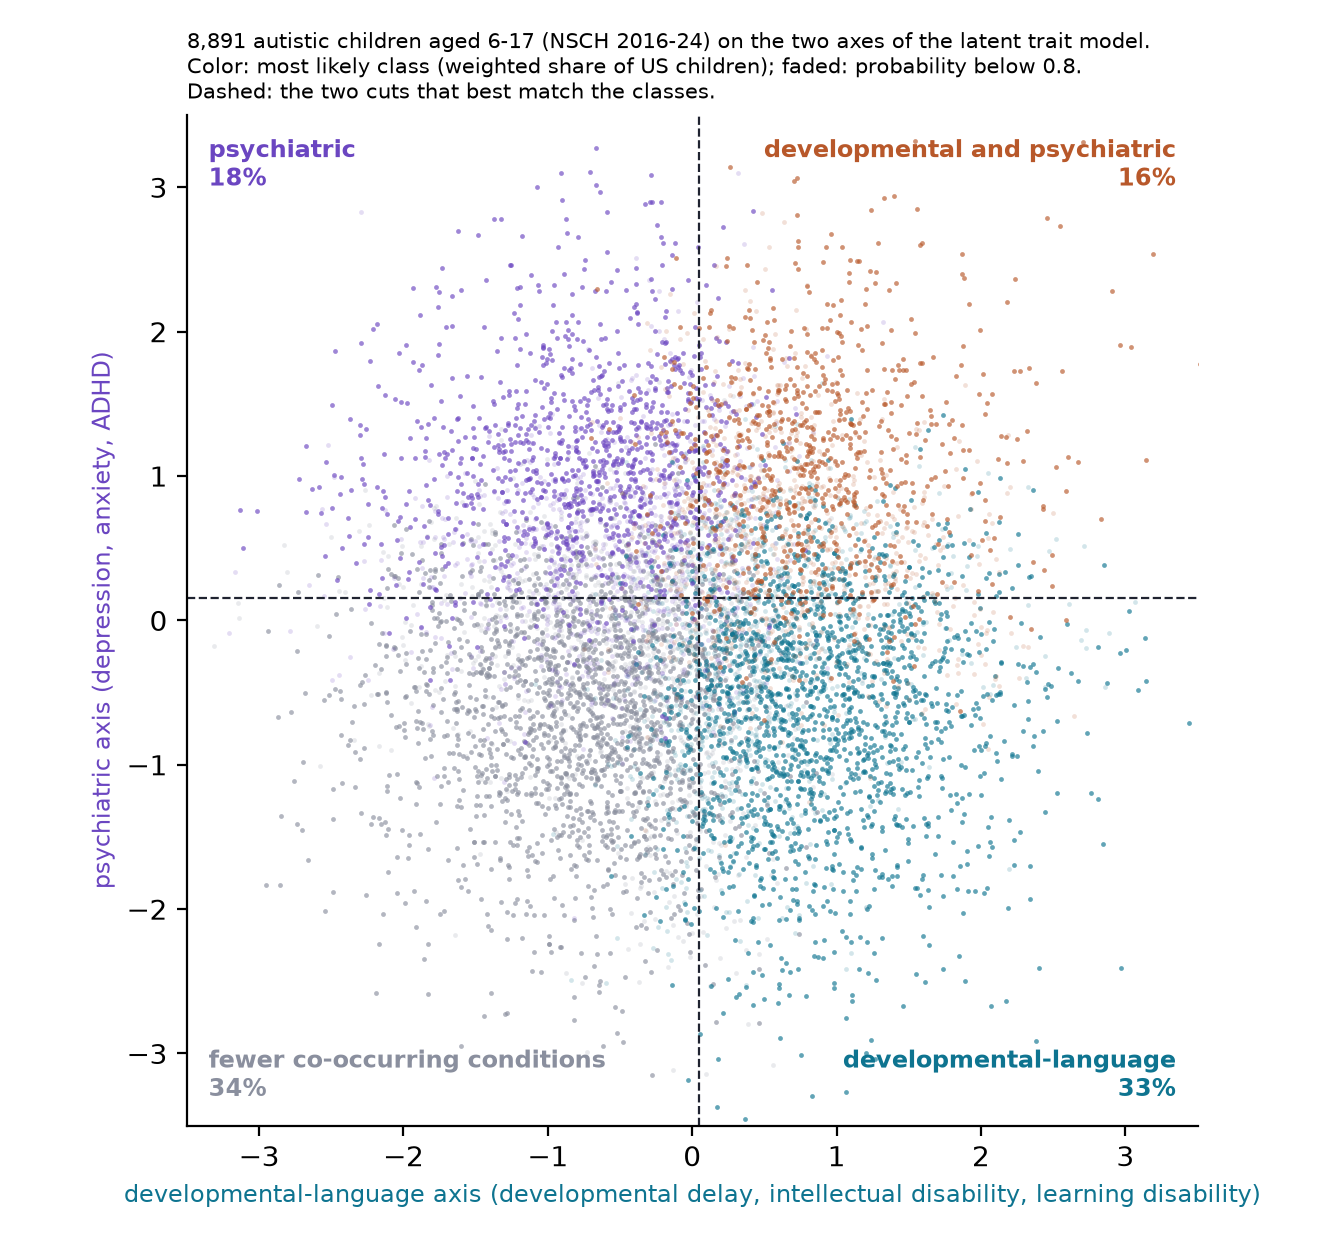
\includegraphics[width=0.62\textwidth]{figure1_map.png}
\caption{The 8,891 children placed on the two axes of the latent trait model (one draw from each child's posterior). Color is the most likely of the four latent classes; children whose largest class probability is below 0.8 are faded. Dashed lines are the two cuts on the axes that best reproduce the classes (ARI 0.80). The corner labels give each class's weighted share of US autistic children aged 6 to 17. The children form one cloud, and the classes are its quadrants.}
\label{fig:map}
\end{figure*}

\subsection{Two axes}
\label{sec:axes}
Figure~\ref{fig:map} shows the result the rest of the section builds toward. The two-dimensional latent trait model separates the 18 conditions into two sets (Figure~\ref{fig:loadings}). A developmental-language axis carries developmental delay (slope 3.97), intellectual disability (3.14), learning disability (2.51), Down syndrome (2.19) and speech or language disorder (2.03), with cerebral palsy and epilepsy more weakly. A psychiatric axis carries depression (3.63), anxiety (2.51), headaches (1.13), ADHD (0.89) and Tourette syndrome (0.87). Behavior problems load on both (0.68 and 0.73). Bootstrap standard errors for the slopes are 0.03 to 0.28, and the same two axes appear when the model is fit separately to ages 6 to 11 and 12 to 17 (congruence 0.98 or higher). The psychiatric position rises with age (correlation 0.26), which matches when anxiety and depression are usually diagnosed, and the developmental position falls slightly ($-0.11$).

The four latent classes of Section~\ref{sec:profiles} are the four combinations of high and low on these axes. Two cuts on the axes, placed at the class means, reproduce the class assignments at ARI 0.80. The children do not form four separate clumps: they form one cloud, and the children whose class is uncertain lie along the cuts.

\begin{figure}[t]
\centering
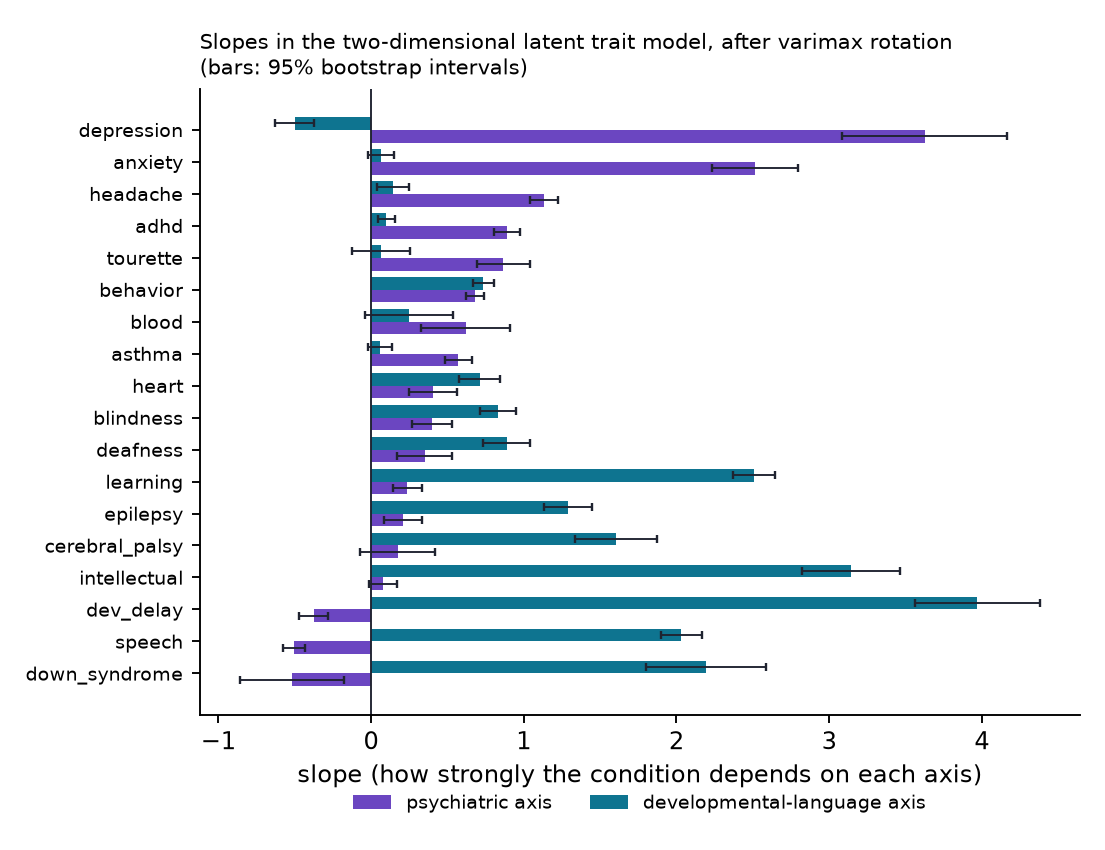
\includegraphics[width=\columnwidth]{loadings.png}
\caption{Slopes of the two-dimensional latent trait model, with 95\% intervals from 50 bootstrap refits. Each condition loads mainly on one axis; behavior problems load on both.}
\label{fig:loadings}
\end{figure}

\subsection{How many classes}
\label{sec:howmany}
BIC fell at every $K$ from 1 to 8, while the shuffled baseline rose throughout, so there is structure, but no $K$ is selected: the drops shrink from 8,224 ($K=1$ to 2) to 6 ($K=7$ to 8), and every class added after $K=5$ holds under 3\% of children. Held-out likelihood also improves through $K=8$ (Table~\ref{tab:models}). By the stability rule, the least stable class has mean Jaccard 0.91 at $K=4$, 0.63 at $K=5$, 0.55 at $K=6$, 0.64 at $K=7$ and 0.58 at $K=8$, so the rule gives $K=4$. The choice does not depend on the threshold or the number of resamples: at thresholds of 0.7, 0.75 and 0.8, with 50, 100 or 200 resamples, $K=4$ is the only $K$ that passes, and it is also the most stable $K$ tested.

The calibration limits what this means. On data simulated from the two-dimensional model, which has no classes, every class is stable through $K=5$ (least stable 0.84 at $K=4$ and 0.88 at $K=5$) and stability breaks only at $K=6$. A smooth cloud can be cut into four or five pieces that come back in every resample, so the rule finds the finest division that reproduces, not the number of groups. On data simulated from the $K=5$ class model all five classes are stable (0.92 or more, including an 8\% class), so the real fifth class does not fail for being small.

\begin{table}[t]
\centering
\caption{Classes against dimensions. BIC on 2016 to 2024; held-out log-likelihood as the difference from the three-dimensional model, the best one that is not degenerate (standard error). $D=4$ ends on the slope bound and is not interpreted.}
\label{tab:models}
\small
\setlength{\tabcolsep}{4pt}
\begin{tabular}{lrrrr}
\toprule
Model & Param. & BIC & 2022--24 & 2025 \\
\midrule
Classes, $K=4$ & 75 & 106,427 & $-286$ (32) & $-106$ (16) \\
Classes, $K=5$ & 94 & 105,959 & $-182$ (25) & $-64$ (13) \\
Classes, $K=8$ & 151 & 105,655 & $-60$ (22) & $-23$ (11) \\
Trait, $D=1$ & 36 & 109,198 & $-1063$ (50) & $-374$ (29) \\
Trait, $D=2$ & 53 & 105,291 & $-57$ (14) & $-26$ (8) \\
Trait, $D=3$ & 69 & 105,095 & 0 & 0 \\
Trait, $D=4$ & 84 & (104,909) & ($+54$) & ($+14$) \\
\bottomrule
\end{tabular}
\end{table}

\subsection{The four profiles}
\label{sec:profiles}

\begin{figure*}[t]
\centering
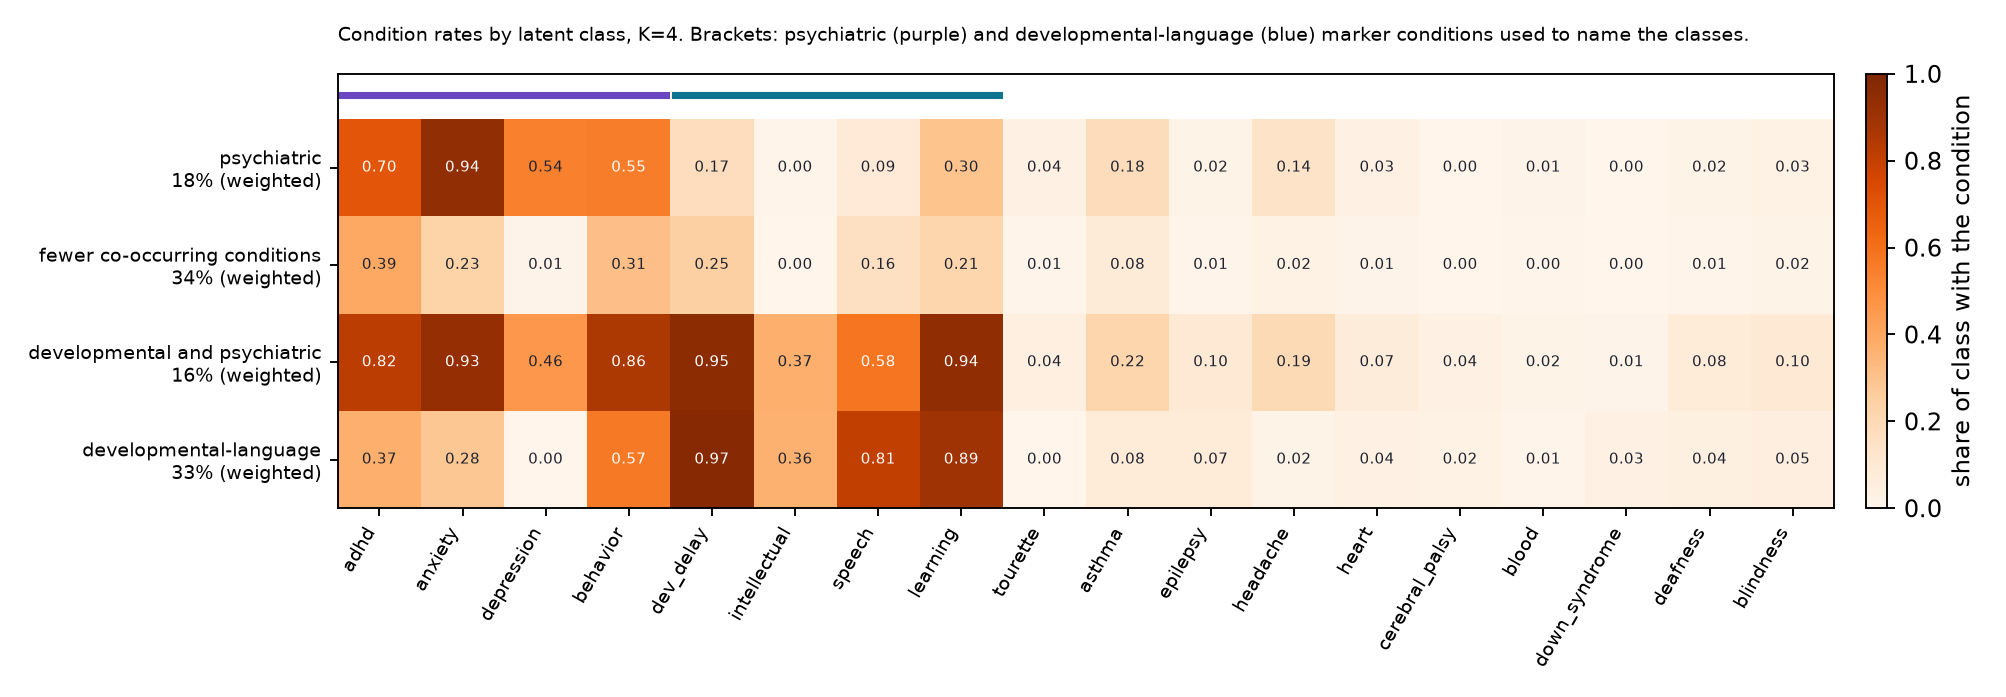
\includegraphics[width=\textwidth]{classes.png}
\caption{Condition rates in the four latent classes ($K=4$), with weighted shares of US autistic children aged 6 to 17. Bars above mark the psychiatric (purple) and developmental-language (blue) conditions used to name the classes.}
\label{fig:classes}
\end{figure*}

\begin{stub}{Haley, about 0.4 column}
Walk through Figure~\ref{fig:classes}. Weighted shares with 95\% intervals (\texttt{results\_k4/shares.csv}): fewer co-occurring conditions 34\% (32 to 36), developmental-language 33\% (31 to 35), psychiatric 18\% (16 to 19), developmental and psychiatric 16\% (14 to 17). Defining rates: developmental-language has developmental delay 0.97, learning 0.89, speech 0.81, intellectual 0.36; psychiatric has anxiety 0.94, ADHD 0.70, depression 0.54; both has ADHD 0.82, anxiety 0.93, behavior 0.86, delay 0.95, learning 0.94; fewer has nothing above 0.39 (ADHD). Medical conditions are low everywhere and highest in the ``both'' class. Age and sex by class (\texttt{results\_k4/demographics.csv}). Assignment certainty: relative entropy 0.72; a quarter of children have no class above 0.7. Shares by year (\texttt{reports/figures/results/shares\_by\_year.png}) stay within their intervals; ``both'' drifts from 19\% in 2016 to 14\% in 2024; 2025 shares within 3.2 points of the pooled shares.
\end{stub}

\subsection{What replicates, and what that shows}
\label{sec:replication}

\begin{figure}[t]
\centering
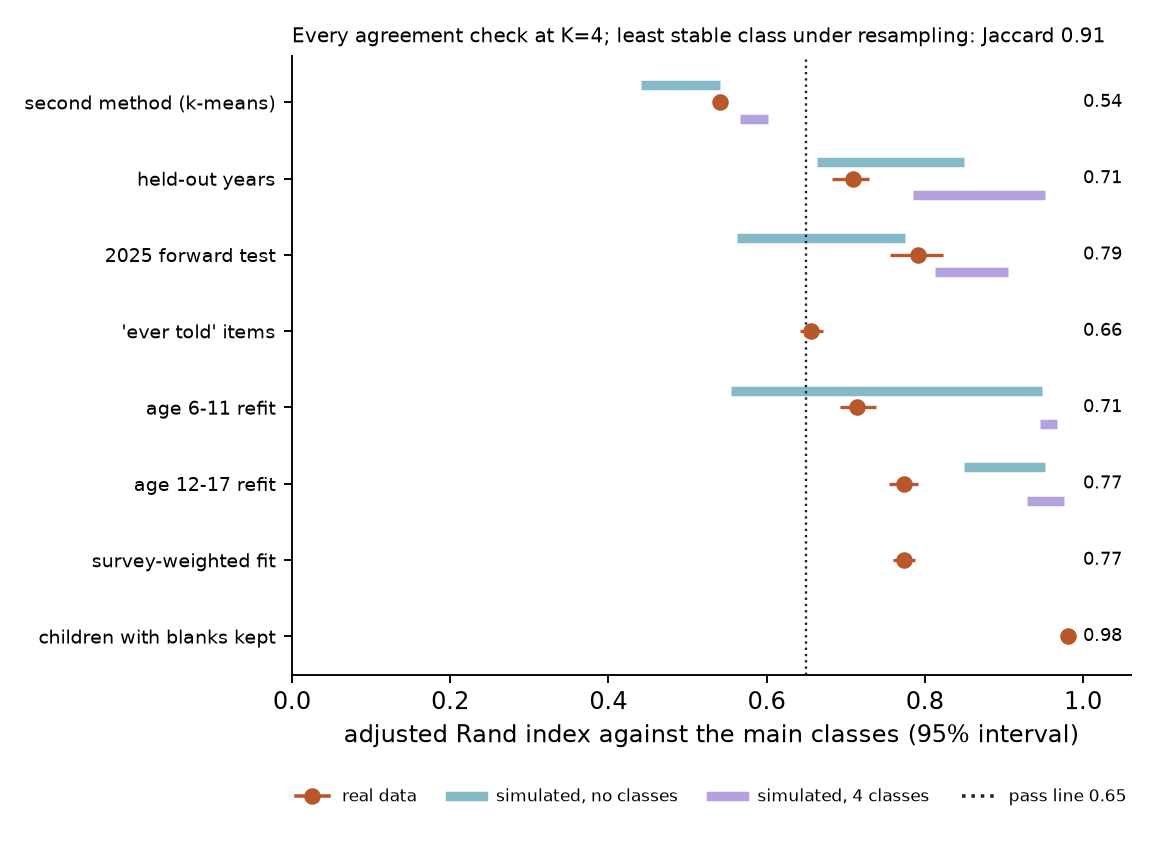
\includegraphics[width=\columnwidth]{checks_k4.png}
\caption{Every agreement check at $K=4$ (dots, with 95\% intervals from resampling children), beside the range the same check gives on five datasets simulated from the two-dimensional model with no classes (teal) and five from the four-class model (lilac). Dotted line: the 0.65 pass line.}
\label{fig:checks}
\end{figure}

Table~\ref{tab:checks} and Figure~\ref{fig:checks} give every check at $K=4$. The classes pass the independent replications: fit separately on 2016 to 2021 and on 2022 to 2024, the two models label the later children at ARI 0.71 (0.68 to 0.73), and the frozen model and a fresh fit agree on the 2025 children at 0.79 (0.76 to 0.82). They pass within each age band (0.71 and 0.77) and under resampling (every class's mean Jaccard 0.91 to 0.93). The ``ever told'' items give 0.66 (0.64 to 0.67), on the line. The survey-weighted fit agrees at 0.77, refits from five other seeds at 1.00, and the refit that keeps the 819 children with blank answers at 0.98, with class sizes within half a point.

The second method fails. $k$-means agrees with the classes at 0.54, and across five seeds its best solutions differ in total distance by about 0.01\% and agree with the classes at 0.52 to 0.58. The disagreement is at the borders: among the 52\% of children the class model places with probability 0.9 or more, $k$-means agrees at 0.93. The proposal's average-linkage hierarchical clustering on Jaccard distance failed outright, putting 94\% of children in one cluster at every $K$ from 4 to 6 (ARI 0.00). With 18 yes/no items, thousands of children sit at small distances from one another, average linkage chains through them, and the 517 children with no conditions form a separate point. Complete linkage, prevalence-weighted Jaccard and spectral clustering do no better (0.08 or less), and Ward linkage reaches 0.34.

\begin{table}[t]
\centering
\caption{Checks at $K=4$: real ARI with its 95\% interval, beside the range over five datasets simulated from the two-dimensional model (no classes) and five from the four-class model. Pass line 0.65.}
\label{tab:checks}
\small
\setlength{\tabcolsep}{3pt}
\begin{tabular}{lccc}
\toprule
Check & Real & Continuum & 4 classes \\
\midrule
Held-out years & 0.71 (0.68--0.73) & 0.66--0.85 & 0.78--0.95 \\
2025 forward test & 0.79 (0.76--0.82) & 0.56--0.78 & 0.81--0.91 \\
Age 6--11 & 0.71 (0.69--0.74) & 0.56--0.95 & 0.95--0.97 \\
Age 12--17 & 0.77 (0.76--0.79) & 0.85--0.95 & 0.93--0.98 \\
$k$-means & 0.54 & 0.44--0.54 & 0.57--0.60 \\
``Ever told'' items & 0.66 (0.64--0.67) & & \\
Weighted fit & 0.77 (0.76--0.79) & & \\
Blanks kept & 0.98 (0.98--0.99) & & \\
\midrule
Bootstrap Jaccard & 0.91 (least) & 0.84 & 0.92$^{a}$ \\
\bottomrule
\end{tabular}
\\[2pt]{\footnotesize $^{a}$ Least stable class in the five-class simulation at $K=5$.}
\end{table}

The calibration changes how these passes read. A four-way cut of the simulated continuum, which has no groups in it, reproduces across held-out years at 0.66 to 0.85, in a fresh 2025-sized sample at 0.56 to 0.78, within age bands at 0.56 to 0.95 and 0.85 to 0.95, and against $k$-means at 0.44 to 0.54. Data with four real classes reproduce better on every check: 0.78 to 0.95 across years, 0.81 to 0.91 in 2025, 0.93 to 0.98 within age bands and 0.57 to 0.60 against $k$-means. The real values sit inside the continuum's range for held-out years, the younger band and $k$-means, just above it for 2025 (0.79 against 0.78) and below it for the older band, and below the four-class range on every check. So the partition is reproducible, as a partition of a continuum also is, and the replication checks cannot by themselves say that its pieces are groups. On every check the real data replicate the way a continuum does.

\subsection{Classes or dimensions}
\label{sec:classes-or-dimensions}
The continuous model describes the data better (Table~\ref{tab:models}, Figure~\ref{fig:fit}). With 53 parameters, $D=2$ has a lower BIC than any class model, including $K=8$ with 151. On held-out years it predicts as well as eight classes: measured from $D=3$, $D=2$ trails by 57 log-likelihood units (standard error 14) on 2022 to 2024 and by 26 (8) on 2025, and $K=8$ by 60 (22) and 23 (11), while $K=4$ trails by 286 and 106. $D=4$ is degenerate: one dimension collapses onto ADHD and its slope runs to the bound.

\begin{figure}[t]
\centering
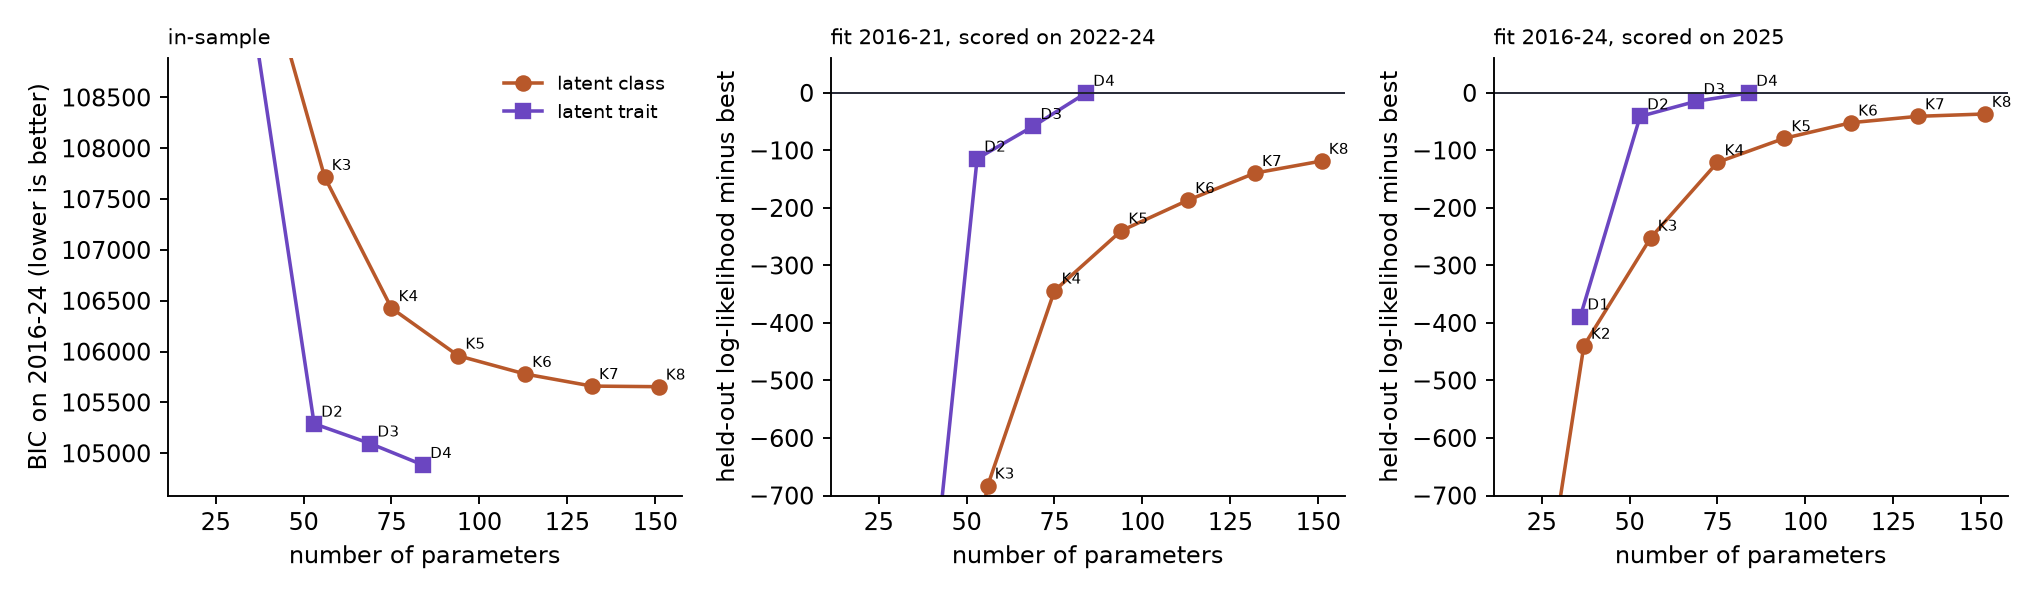
\includegraphics[width=\columnwidth]{model_fit.png}
\caption{In-sample BIC and held-out log-likelihood for latent class models ($K=1$ to 8) and latent trait models ($D=1$ to 4). $D=4$ (hollow) ends on the slope bound.}
\label{fig:fit}
\end{figure}

Three further results point the same way. Data simulated from the fitted $D=2$ model give a class BIC curve that keeps falling through $K=6$, as the real one does, while data simulated from four classes give a curve that turns up at $K=4$, so this comparison can tell the two apart and the real data behave like the continuum \citep{bauer2004}. The model with three dimensions adds a medical-sensory axis (cerebral palsy, deafness, blindness, Down syndrome, epilepsy, headaches) and cuts the pairs of conditions with poor fit from 49 to 36 of 153; pairs such as deafness with blindness and epilepsy with cerebral palsy are among those the $K=4$ and $D=2$ models fit worst. And the estimated distribution of positions is not a bell curve: it improves on the normal by 94 log-likelihood units, against 16 to 22 for data simulated from the continuum and 180 to 199 for data from four classes. The real children are lumpier than a smooth cloud and about half as lumpy as four separate groups, which is the pattern a factor mixture model would describe.

\subsection{Severity}
\label{sec:severity}

\begin{figure}[t]
\centering
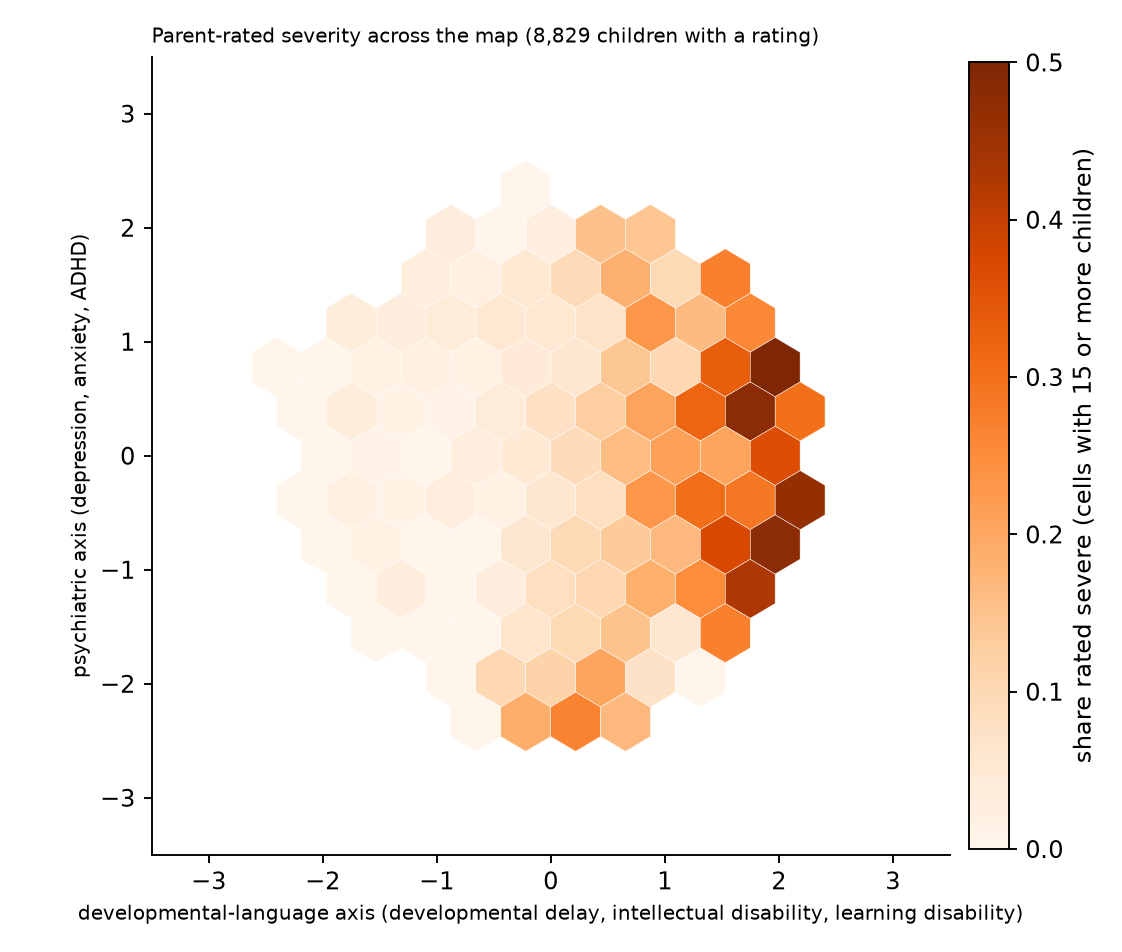
\includegraphics[width=\columnwidth]{severity_map.png}
\caption{Share of children rated severe across the map of Figure~\ref{fig:map} (hexagons with 15 or more children). Severity rises along the developmental-language axis and does not jump at the class borders.}
\label{fig:severity}
\end{figure}

\begin{stub}{Haley, about 0.4 column}
Severity by class (\texttt{results\_k4/severity\_by\_class.csv}, \texttt{reports/figures/results/severity\_by\_class.png}): rated severe 21\% in developmental-language and in both, 2\% in fewer, 4\% in psychiatric. Figure~\ref{fig:severity}: rises along the developmental axis, no jump at the borders. The planned test (\texttt{results\_k4/count\_vs\_class.csv}): count plus class beats count on BIC (14,447 against 14,873) and log-loss (0.815 against 0.840); class alone does not (BIC 14,996; log-loss 0.846). So the classes pass on one reading of the pre-fit sentence and fail on the other. Comparators: class probabilities 14,622; the two factor scores alone 14,262 with 6 parameters, better than count plus class; scores plus class 14,243; all 18 flags 14,159. Severity and flags come from the same parent in one interview, so part of any association is shared reporting style; model comparisons are less affected than any single association.
\end{stub}

\subsection{Five classes}
\label{sec:k5}
\begin{stub}{Haley, about 0.25 column}
$K=5$ (\texttt{results\_k5/}): adds a class with intellectual disability, speech and developmental delay near 1 and the highest rates of epilepsy, cerebral palsy, Down syndrome, deafness and blindness; 9\% weighted, 45\% rated severe. It appears in every resample but its membership does not hold (Jaccard 0.63); held-out years fail (ARI 0.635, 0.62 to 0.65); weighted fit disagrees (0.59); 2025 0.78 and age bands 0.79 and 0.85 pass. Same signal as the third (medical-sensory) dimension. Corresponds to the ``broadly affected'' groups of \citet{vargason2019} (24\%) and \citet{litman2025} (10\%). Past $K=5$ the replication and 2025 tests fail too (\texttt{reports/tables/checks\_by\_k.csv}).
\end{stub}

\section{Discussion}
\label{sec:discussion}

\begin{stub}{Haley first draft, then both; about 1.5 columns}
\emph{What was found}, in three beats: the four profiles are there and reproduce; they reproduce the way a cut continuum does; severity follows the developmental axis, not class. Two dials, not four boxes (\texttt{docs/team-notes.md} has the short version).

\emph{Against the literature.} The contrasts clinic studies report (developmental, psychiatric, high burden, few conditions) appear in a national sample, as quadrants of two axes. Litman et al.'s 37/19/34/10 against our 18/33/34/16 \citep{litman2025}; their ``broadly affected'' class and Vargason's high-rate group \citep{vargason2019} match our unstable $K=5$ class. \citet{zhang2025}'s two genetic factors as the counterpart of our two axes, including the age pattern (psychiatric position rises with age). \citet{kim2019} and \citet{wittkopf2023} reached dimensional or hybrid answers for core traits; ours is the first such comparison for co-occurring conditions that we found. The latent density result (lumpier than a bell curve, half as lumpy as four groups) fits the hybrid reading.

\emph{What replication can show.} The calibration is the methodological point: held-out-year, forward and age-band replication pass for a partition of a smooth continuum, so passing them is necessary but not sufficient evidence of subtypes. Other studies relying on these checks could run the same simulation.

\emph{Why distance methods fail on sparse binary items}: chaining in average linkage, near-tied $k$-means optima; what that means for cross-method replication as a criterion.

\emph{Limitations.} Parent report of a provider's diagnosis, so access to care and diagnostic practice are in the flags; one observation per child, so no temporal or predictive validation; entropy 0.72; 8.4\% with blank answers (refit says it does not matter); ``currently has'' wording; the $K$ rule was set after seeing results and the 2025 test is confirmatory; the proposal's hierarchical method failed and was replaced; severity and flags share an informant.

\emph{Next.} A factor mixture model \citep{lubke2005}, which allows classes and continuous variation within them; three-step corrections for relating classes to outcomes \citep{vermunt2010}.

\emph{For a clinician}: describe a child by where they sit on two dials rather than which of four boxes; severity ratings track the developmental dial.
\end{stub}

\section{Reproducibility}
\label{sec:repro}
All code is at \url{https://github.com/Naalu/nsch-autism-subtypes} under the MIT license. The pipeline downloads the public Census files, builds the analysis table and runs fifteen numbered scripts, each with a fixed seed; \texttt{make all} reproduces every number and figure in this paper, and \texttt{make paper} builds it. The latent class model, average-linkage hierarchical clustering, $k$-means and the latent trait model are our NumPy implementations; the first three are tested against StepMix, SciPy and scikit-learn, and every class-model step can be rerun with those libraries in place of our code (\texttt{--backend reference}). The processed analysis table and codebook are committed, dependency versions are locked, and continuous integration runs the tests on every change. The data are public and deidentified, and no IRB review was required.


{\small
\bibliographystyle{plainnat}
\bibliography{references}
}

\end{document}
